\documentclass{article}
\usepackage[utf8]{inputenc} % per le lettere accentate
\usepackage{graphicx} % per l'inserimento di immagini e grafici
\usepackage{booktabs} % per gestire le tabelle
\usepackage{amsmath}
\usepackage{float}
\usepackage{subfig}
\usepackage{enumerate}
\newcommand{\e}[1]{\cdot 10^{#1}} % definisco un nuovo comando per poter scrivere la notazione scientifica rapidamente

\begin{document}
%\SweaveOpts\ref{concordance=TRUE}
\author{Simone Brazioli}
\title{Primo Esercizio per Esame di Calcolo per l'Astronomia}
\date{A.A. 2019-2020}

\maketitle
\begin{abstract}
In questa relazione mostrerò l'analisi richiesta delle curve di luce
di un catalogo di stelle Cefeidi per ottenere una stima della Costante
di Hubble. Utilizzerò questa costante per calcolare un'approssimazione
dei parametri cosmologici $\Omega_M$ e $\Omega_\Lambda$ nelle
assunzioni di Universo Piatto, Chiuso o Aperto.
\end{abstract}

\tableofcontents
\clearpage

\section{Introduzione}
Il problema dell'età dell'Universo e delle sue caratteristiche
fondamentali, ha impegnato per secoli gli scienziati e prima di loro i
filosofi.

Fino a inizio '900, l'idea più quotata era che l'universo fosse finito
e statico, immobile. In buona sostanza si identificava la Via Lattea,
la galassia in cui risiede il Sole con il suo sistema, come l'intero
Universo.

Fu nei primi decenni del '900 che le opinioni cambiarono
radicalmente. Spinto infatti dalle nuove scoperte osservative di
\textbf{Henrietta Leavitt} e teoriche di \textbf{Lemaître} e
\textbf{Einstein}, l'astronomo statunitense \textbf{Hubble} determinò
sperimentalmente che l'universo non solo era molto più grande di
quanto si pensasse (di fatto, la Via Lattea non è che una delle mille
miliardi di galassie nell'Universo), ma anche che l'Universo fosse in
espansione.

\subsection{Relazione Periodo-Luminosità delle Cefeidi}
Le Cefeidi sono stelle di età avanzata e massa intermedia che
attraversano una fase instabile del loro ciclo evolutivo. Questa fase
instabile si manifesta in una pulsazione dell'intera stella. Esse,
infatti, si contraggono ed espandono a ritmi regolari nel tempo (per
certi casi anche con un periodo dell'ordine delle ore).

Questa contrazione ed espansione determinano una variazione della
loro luminosità. Per questo vengono classificate come stelle
variabili.

A inzio '900, l'Astronoma Henrietta Leavitt, analizzando le lastre
fotografiche della Piccola e Grande Nube di Magellano (\emph{SMC} e
\emph{LMC}) compilò un catalogo di 1777 stelle variabili periodiche e
ne classificò 47 di queste come Cefeidi.

Misurando il periodo delle loro variabilità, notò che le Cefeidi con
un periodo più lungo risultavano essere più brillanti di quelle con un
periodo più corto. Dato che queste stelle appartenevano tutte alla
stessa nube, e quindi si trovavano a una distanza grosso modo uguale
dall'osservatore, questa differenza in magnitudine apparente
rispecchiava anche una differenza in magnitudine assoluta.

Fu così che, graficando separatamente le curve di luce delle Cefeidi
per le due nubi, Henrietta Leavitt si accorse della presenza di
un'effettiva relazione tra Periodo e Luminosità.

\begin{figure}[H]
  \centering
  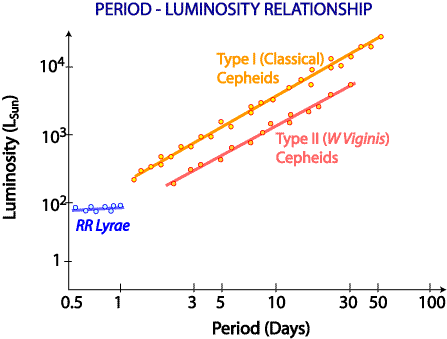
\includegraphics[width=.5\textwidth]{plrelnceph}
  \caption{Relazione Periodo-Luminosità per Cefeidi e RR Lyrae.}
\end{figure}

Matematicamente, questa relazione possiamo esprimerla come:
\begin{equation}
  M_V = c_1 \log (P) + c_2
\end{equation}

Grazie a questa relazione, possiamo usare le Cefeidi per stimare la
distanza di oggetti nella nostra galassia e negli ammassi, fino alle
galassie più vicine, come \textbf{M31}.

Il metodo delle Cefeidi è diventato, inoltre, un importantissimo
metodo di calibrazione per altre metodologie di calcolo delle distanze
per oggetti più lontani.

\clearpage

\subsection{La Legge di Hubble Lemaître}

La Legge di Hubble-Lemaître venne derivata indipendentemente da
Lemaître a livello teorico e da Hubble a livello osservativo nei primi
anni del '900.

Sfruttando le stelle Cefeidi (e la loro relazione di Leavitt) nelle galassie più vicine alla Via
Lattea, infatti, Hubble fu in grado di stimare le distanze e mostrare
come l'Universo fosse più grande di quanto si pensasse. Inoltre,
studiando gli spettri della luce proveniente da queste stelle e da queste galassie,
notò che presentavano un \textbf{redshift}, cioè uno spostamento verso
il rosso. Tale redshift viene fisicamente interpretato come effetto \emph{Doppler}.\footnote{In realtà, il primo caso in studio di Hubble fu
  \emph{M31} che mostrava un \textbf{blueshift}.}
Questo redshift, indicava che le galassie si stavano spostando nei
confronti dell'osservatore (Sistema Solare e per estensione la Via
Lattea). Osservando risultati e redshift più accentuati per altre galassie più lontane,
Hubble capì che vi era una relazione di proporzionalità diretta tra la
distanza di una galassia (calcolabile grazie alla relazione
Periodo-Luminosità delle Cefeidi) e la sua velocità di recessione
(misurabile tramite redshift nello spettro). Fu così che nacque la
Legge di Hubble\footnote{Lemaître aveva già derivato, in linea teorica, tale equazione (come
conseguenza della Relatività Generale di Einstein), ma storicamente
Hubble venne considerato il suo scopritore. Solo nel 2019, la
\emph{IAU} decise di 'rinominare' la Legge includendo Lemaître.}:

\begin{equation}
  v_{rec} = H_0 d
\end{equation}

Importante in questa equazione è la Costante di Hubble $H_0$ che fissa
la scala delle distanze e dei tempi nella cosmologia.
\clearpage

\subsection{La Legge di H-L nella Cosmologia}

La Costante di Hubble è una delle costanti fondamentali della
cosmologia. Grazie a questa costante possiamo effettuare una stima
dell'età del nostro Universo. Infatti la costante di Hubble ha le
dimensioni del reciproco di un tempo e viene misurata comunemente in
$\frac{km}{s\cdot Mpc}$. Invertendo, quindi, la costante di Hubble (e
aggiustando le unità di misura posso ottenere una stima dell'età
dell'Universo.

\begin{equation}
  t_{0,h} = \frac{1}{H_0}
\end{equation}


Questa, tuttavia, è una sovrastima che deve essere corretta. In
cosmologia, infatti, l'età dell'Universo si può calcolare tramite:

\begin{equation}
  t_0 = \int_0^{t_0} dt = \frac{1}{H_0} \int_0^\infty \frac{dz}{\left
      ( 1+z \right ) E\left ( z \right ) ^{1/2}}
\end{equation}

dove

\begin{equation}\label{eqn:time}
  E\left ( z \right ) = \Omega_M \left ( 1+z \right ) ^3 + \left ( 1
    - \Omega_M - \Omega_\Lambda \right ) \left ( 1+z \right ) ^2
  +\Omega_\Lambda
\end{equation}

In queste espressioni, i parametri $\Omega_M$ e $\Omega_\Lambda$ sono
parametri cosmologici che dipendono dal modello di Universo che si sta
considerando. In particolare:

\begin{equation*}
  \Omega = 
  \begin{cases}
    \Omega_M + \Omega_\Lambda = 1 \qquad \hbox{nel caso di
      Universo Piatto - Geometria Euclidea} \\
    \Omega_M + \Omega_\Lambda < 1 \qquad \hbox{nel caso di
      Universo Aperto - Geometria Iperbolica} \\
    \Omega_M + \Omega_\Lambda > 1 \qquad \hbox{nel caso di
      Universo Chiuso - Geometria Sferica}
  \end{cases}
\end{equation*}

$\Omega$ parametrizza la densità dell'Universo rapportata alla densità
critica\footnote{definita come la densità di materia/energia che deve
  avere l'Universo affinchè abbia una geometria euclidea (cioè
  piatta).}.

\clearpage
\section{Dati Disponibili}



L'esercizio offre un database (\emph{data/ceph\_catalog.txt}) di stelle cefeidi già analizzate per le quali viene data la
Magnitudine Assoluta e il Periodo di Pulsazione. Da questo database,
bisogna ricavare i coefficienti $c_1$ e $c_2$ della relazione
Periodo-Luminosità vista in precedenza.

In aggiunta, ho un set di dati osservativi (\emph{data/ceph\_NGC*.txt}) che mostrano l'andamento
della magnitudine apparente di 19 stelle Cefeidi (appartenenti ad
altrettante galassie) in funzione del tempo (\emph{Julian Day}). Tuttavia, tali dati non
sono ordinati temporalmente. Da questi dati, una volta ridotti, ricavo
le curve di luce, tramite integrazione, che mi permettono di fare
delle stime della lunghezza del periodo. Da queste stime di periodo,
ottengo una approssimazione della magnitudine assoluta.

Una volta ottenuta la magnitudine assoluta posso derivare la distanza
delle galassie che ospitano le Cefeidi analizzate. Ho a disposizione
un file (\emph{data/gal\_vel .txt}) che mi mostra, per ciascuna delle galassie in cui ho una
Cefeide, una misura della \emph{velocità di recessione} con relativo
errore. Da questi dati, sfruttando la Legge di Hubble, ottengo una
misura della costante di Hubble.

Una volta conosciuta la stima della costante di Hubble e del relativo
errore, posso studiare, con l'equazione (\ref{eqn:time}) vista in
precedenza, l'andamento dell'età dell'universo in funzione della
scelta dei parametri $\Omega_\Lambda$ e $\Omega_M$. Imponendo di
ottenere la misura dell'età dell'Universo data dalla missione Planck,
cioè
\begin{equation*}
  t_0 = 13.82 \pm 0.1382
\end{equation*}

cerco una coppia di parametri $\Omega_i$ per ciascuno dei tre modelli
di universo considerabili: Universo Piatto, Universo Aperto, Universo
Chiuso.

Alla fine confronto i parametri ottenuti (nel caso di Geometria
Piatta) con gli $\Omega_i$ comunemente accettati dalla comunità scientifica.

\clearpage
\section{Algoritmi Numerici Utilizzati in FORTRAN}

Il cuore del codice è l'algoritmo di interpolazione numerica delle
curve di luce. Infatti, una volta ordinati, i file contenenti le curve
di luce hanno un andamento discreto, sul quale una stima del periodo è
molto grossolana.

Per poter aumentare la precisione delle analisi, ho scelto di implementare un
algoritmo di interpolazione tramite \emph{spline cubica}.

\subsection{Spline Cubica}

Nella Spline Cubica, ciascun intervallo tra due osservazioni viene
rappresentato da un diverso polinomio al terzo ordine:

\begin{equation}
  f_k(x) = a_{k,i} x^3 + b_{k,i} x^2 + c_{k,i} x + d_{k,i}
\end{equation}

Come condizioni di interpolazione abbiamo le seguenti:

\begin{equation}
  \begin{cases}
    f_k(x_k) = y(k) \\
    f_{k} (x_{k+1}) = f_{k+1} (x_{k+1}) \\
    \dot f_{k} (x_{k+1}) = \dot f_{k+1} (x_{k+1} )  \\
    \ddot f_{k} (x_{k+1}) = \ddot f_{k+1} (x_{k+1} ) \\
    \ddot f_1(x_1) = 0 = \ddot f_n(x_n) \\
  \end{cases}
\end{equation}

Vale a dire:
\begin{enumerate}
\item la cubica $k$-esima deve passare per il dato $k$-esimo; \\
\item cubiche adiacenti devono unirsi in corrispondenza dei dati; \\
\item nei punti di incontro, due cubiche devono avere la stessa
  derivata prima (pendenza)... \\
\item e la stessa derivata seconda ('flessione');
\item nei nodi finali, la derivata seconda deve essere nulla
  (\emph{spline naturale})
\end{enumerate}

Dopo aver interpolato le curve di luce, posso analizzare quanto
calcolato alla ricerca dei periodi. Utilizzo il passaggio dei dati dal
punto medio per garantire una precisione maggiore dei periodi
calcolati.

Per fare ciò, dapprima identifico, usando i valori discreti forniti dal file originale, l'intervallo in
cui mi aspetto ci sia il passaggio preciso. Dopodichè, ricerco
usando i dati interpolati, all'interno di questo intervallo, il
passaggio dal punto medio.
Faccio in questo modo per evitare di
considerare passaggi spuri dovuti alla rumorosità dei dati o a
imprecisioni di interpolazione.

Riporto nella sezione (\ref{result}) i risultati ottenuti per le
singole cefeidi.

\subsection{Calcolo dei Parametri Cosmologici}

Per calcolare i parametri cosmologici, in funzione del tipo di
universo, tali che riproducesserò l'età stimata dalla missione Planck,
mi sono servito di un algoritmo di integrazione numerica per aggredire
l'integrale visibile nell'equazione (\ref{eqn:time}). In particolare
ho usato un'implementazione della \textbf{quadratura di Gauss a
  quattro punti}.

Se le formule di Newton-Cotes utilizzano la stima della funzione in
punti determinati della funzione (per esempio, gli estremi
dell'intervallo scelto), la quadratura di Gauss si serve di punti
scelti in maniera 'intelligente', per questo viene detto
\emph{metodo dei coefficienti indeterminati}.

Generalizzando la formula dell'integrale tramite trapezoide per
quattro punti, possiamo
scrivere che l'integrale $I$:
\begin{equation}
  I \sim c_0 f(x_0) + c_1 f(x_1) + c_2 f(x_2) + c_3 f(x_3)
\end{equation}

dove $x_i$ sono punti incogniti interni all'intervallo di
integrazione e $c_i$ sono opportuni coefficienti da
determinare. Il tutto corrisponde, quindi, a un equazione con $8$
incognite da calcolare.

Le otto condizioni da applicare per utilizzare l'algoritmo sono
tabulate nelle slide del corso e portano a :

\begin{equation}
  \begin{cases}
    x_{0,1} = \pm \sqrt{\frac{3}{7} - \frac{2}{7}\sqrt{\frac{6}{5}}}
    \\
    x_{2,3} = \pm \sqrt{\frac{3}{7} + \frac{2}{7}\sqrt{\frac{6}{5}}}
    \\
    c_{0,1}  = \frac{18 + \sqrt{30}}{36}\\
    c_{2,3} = \frac{18 - \sqrt{30}}{36}
    \end{cases}
  \end{equation}

  Utilizzando questo algoritmo sono in grado di calcolare l'integrale
  in (\ref{eqn:time}) per ciascuna coppia di parametri cosmologici e
  confrontare con il dato 'vero' per scartare o tenere il risultato.

  \clearpage
  
\section{Risultati}\label{result}

\subsection{Coefficienti Relazione Periodo-Luminosità delle Cefeidi}

Analizzando il set di Cefeidi già analizzate, ho determinato i
seguenti coefficienti $c_1$ e $c_2$:

\begin{center}
 \begin{tabular}{cc}
  \toprule
  $c_1$ & $c_2$ \\
  \midrule
  $-2.90$ & $-1.21$\\
  \bottomrule
 \end{tabular}
\end{center}

\subsection{Curve di Luce delle Cefeidi da Analizzare}

Riporto di seguito, le curve di luce e i periodi e le magnitudini calcolati (con
relativi errori) delle Cefeidi date da analizzare\footnote{Identifico,
  di seguito, le Cefeidi analizzate con la galassia che le ospita, per
  semplificare la notazione.}.
\paragraph{NGC 0925}
\begin{center}
  \begin{tabular}{cccc}
  \toprule
  Periodo Medio ($JD$) & Errore Periodo ($JD$) & M. Apparente Media &
                                                                  Errore
                                                                      su
                                                                      M.A. \\
  \midrule
  $11.37$ & $2.54\e{-2}$ & $25.54$ & $1.95\e{-1}$ \\
  \bottomrule
 \end{tabular}
\end{center}

\begin{figure}[H]
  \centering
  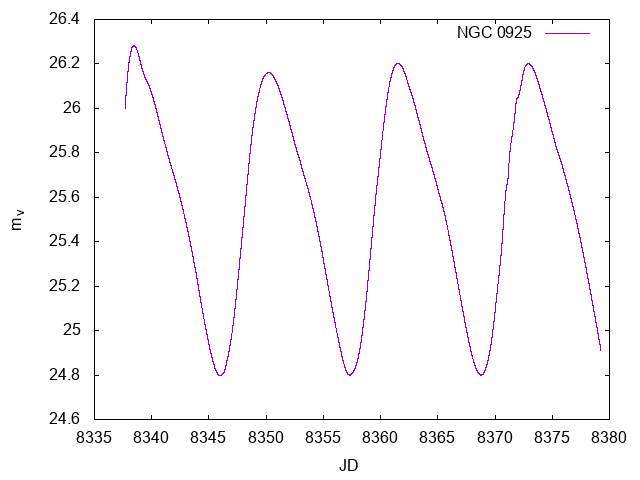
\includegraphics[width=.7\textwidth]{Codice/data/01_NGC0925.png}
  \caption{Curva di Luce della Cefeide in NGC0925.}
\end{figure}

\paragraph{NGC 1326}
\begin{center}
  \begin{tabular}{cccc}
  \toprule
  Periodo Medio ($JD$) & Errore Periodo ($JD$) & M. Apparente Media &
                                                                  Errore
                                                                      su
                                                                      M.A. \\
  \midrule
  $8.67$ & $4.86\e{-2}$ & $27.12$ & $5.28\e{-2}$ \\
  \bottomrule
 \end{tabular}
\end{center}

\begin{figure}[H]
  \centering
  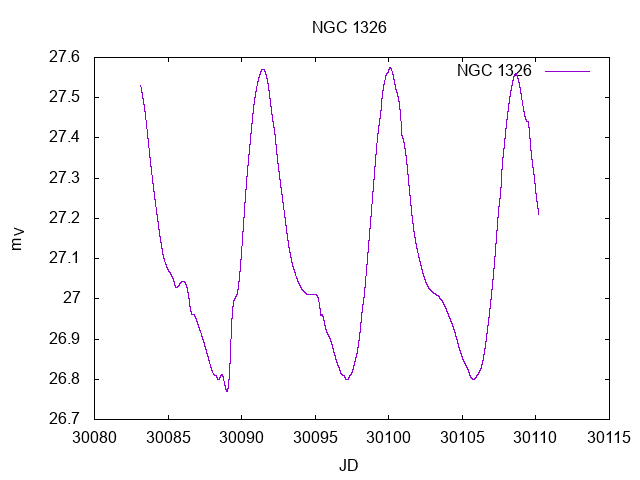
\includegraphics[width=.7\textwidth]{Codice/data/02_NGC1326.png}
  \caption{Curva di Luce della Cefeide in NGC1326.}
\end{figure}

\paragraph{NGC 1365}
\begin{center}
  \begin{tabular}{cccc}
  \toprule
  Periodo Medio ($JD$) & Errore Periodo ($JD$) & M. Apparente Media &
                                                                  Errore
                                                                      su
                                                                      M.A. \\
  \midrule
  $21.31$ & $0.17$ & $26.20$ & $6.46\e{-2}$ \\
  \bottomrule
 \end{tabular}
\end{center}

\begin{figure}[H]
  \centering
  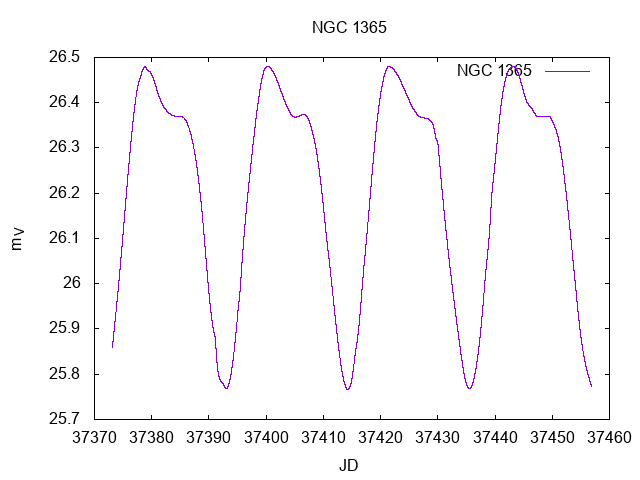
\includegraphics[width=.7\textwidth]{Codice/data/03_NGC1365.png}
  \caption{Curva di Luce della Cefeide in NGC1365.}
\end{figure}

\paragraph{NGC 1425}
\begin{center}
  \begin{tabular}{cccc}
  \toprule
  Periodo Medio ($JD$) & Errore Periodo ($JD$) & M. Apparente Media &
                                                                  Errore
                                                                      su
                                                                      M.A. \\
  \midrule
  $10.74$ & $1.97\e{-2}$ & $27.5$ & $1.70\e{-1}$ \\
  \bottomrule
 \end{tabular}
\end{center}

\begin{figure}[H]
  \centering
  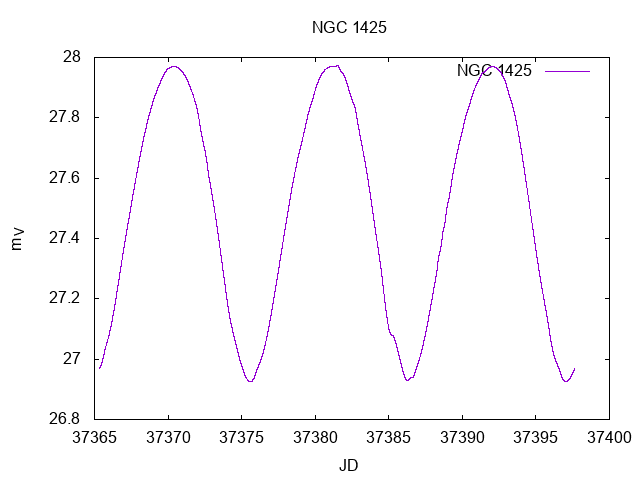
\includegraphics[width=.7\textwidth]{Codice/data/04_NGC1425.png}
  \caption{Curva di Luce della Cefeide in NGC1425.}
\end{figure}

\paragraph{NGC2403}
\begin{center}
  \begin{tabular}{cccc}
  \toprule
  Periodo Medio ($JD$) & Errore Periodo ($JD$) & M. Apparente Media &
                                                                  Errore
                                                                      su
                                                                      M.A. \\
  \midrule
  $3.80$ & $8.99\e{-3}$ & $24.66$ & $3.48e{-1}$ \\
  \bottomrule
 \end{tabular}
\end{center}

\begin{figure}[H]
  \centering
  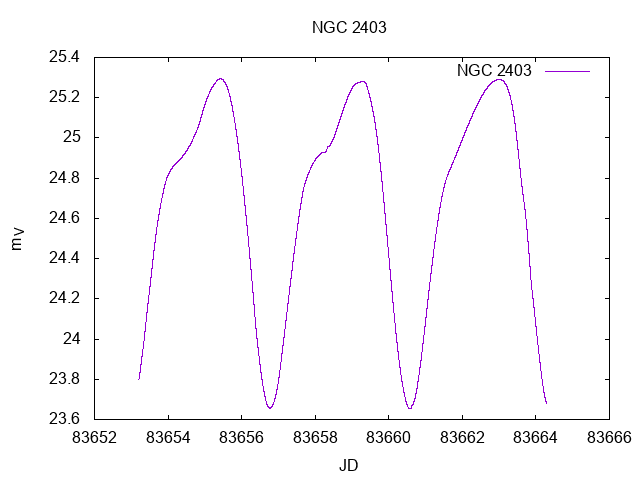
\includegraphics[width=.7\textwidth]{Codice/data/05_NGC2403.png}
  \caption{Curva di Luce della Cefeide in NGC2403.}
\end{figure}

\paragraph{NGC2541}
\begin{center}
  \begin{tabular}{cccc}
  \toprule
  Periodo Medio ($JD$) & Errore Periodo ($JD$) & M. Apparente Media &
                                                                  Errore
                                                                      su
                                                                      M.A. \\
  \midrule
  $19.44$ & $3.03\e{-1}$ & $25.29$ & $1.28\e{-1}$ \\
  \bottomrule
 \end{tabular}
\end{center}

\begin{figure}[H]
  \centering
  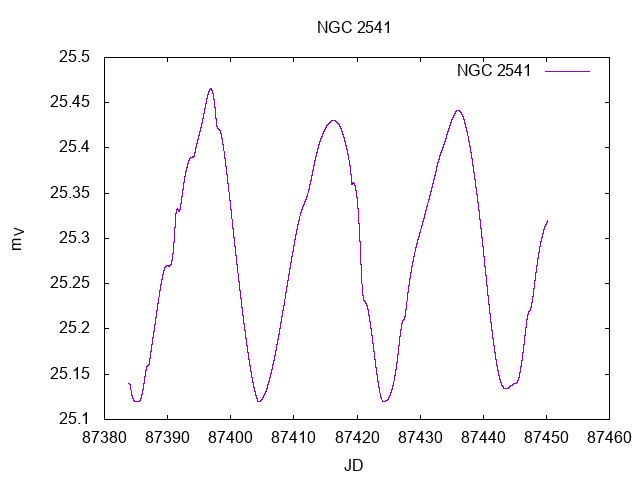
\includegraphics[width=.7\textwidth]{Codice/data/06_NGC2541.png}
  \caption{Curva di Luce della Cefeide in NGC2541.}
\end{figure}

\paragraph{NGC 2090}
\begin{center}
  \begin{tabular}{cccc}
  \toprule
  Periodo Medio ($JD$) & Errore Periodo ($JD$) & M. Apparente Media &
                                                                  Errore
                                                                      su
                                                                      M.A. \\
  \midrule
  $22.43$ & $3.18\e{-2}$ & $25.22$ & $1.69\e{-1}$ \\
  \bottomrule
 \end{tabular}
\end{center}

\begin{figure}[H]
  \centering
  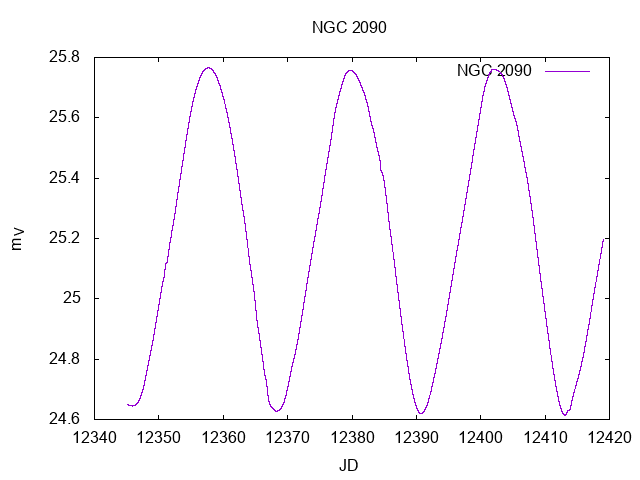
\includegraphics[width=.7\textwidth]{Codice/data/07_NGC2090.png}
  \caption{Curva di Luce della Cefeide in NGC2090.}
\end{figure}

\paragraph{NGC 3198}
\begin{center}
  \begin{tabular}{cccc}
  \toprule
  Periodo Medio ($JD$) & Errore Periodo ($JD$) & M. Apparente Media &
                                                                  Errore
                                                                      su
                                                                      M.A. \\
  \midrule
  $15.12$ & $7.05\e{-2}$ & $26.07$ & $2.32\e{-1}$ \\
  \bottomrule
 \end{tabular}
\end{center}

\begin{figure}[H]
  \centering
  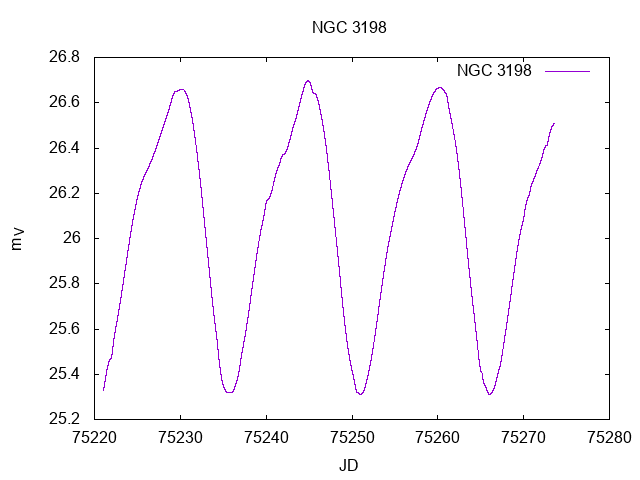
\includegraphics[width=.7\textwidth]{Codice/data/08_NGC3198.png}
  \caption{Curva di Luce della Cefeide in NGC3198.}
\end{figure}

\paragraph{NGC 3351}
\begin{center}
  \begin{tabular}{cccc}
  \toprule
  Periodo Medio ($JD$) & Errore Periodo ($JD$) & M. Apparente Media &
                                                                  Errore
                                                                      su
                                                                      M.A. \\
  \midrule
  $8.20$ & $1.59\e{-2}$ & $26.14$ & $4.87\e{-1}$ \\
  \bottomrule
 \end{tabular}
\end{center}

\begin{figure}[H]
  \centering
  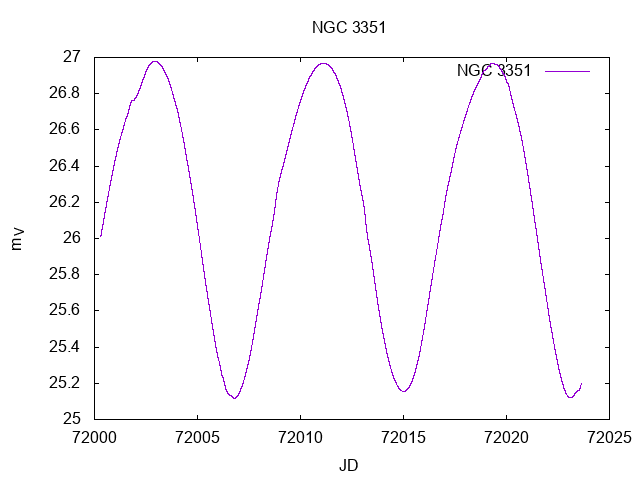
\includegraphics[width=.7\textwidth]{Codice/data/09_NGC3351.png}
  \caption{Curva di Luce della Cefeide in NGC3351.}
\end{figure}

\paragraph{NGC 3368}
\begin{center}
  \begin{tabular}{cccc}
  \toprule
  Periodo Medio ($JD$) & Errore Periodo ($JD$) & M. Apparente Media &
                                                                  Errore
                                                                      su
                                                                      M.A. \\
  \midrule
  $7.73$ & $5.37\e{-2}$ & $26.33$ & $2.88\e{-1}$ \\
  \bottomrule
 \end{tabular}
\end{center}

\begin{figure}[H]
  \centering
  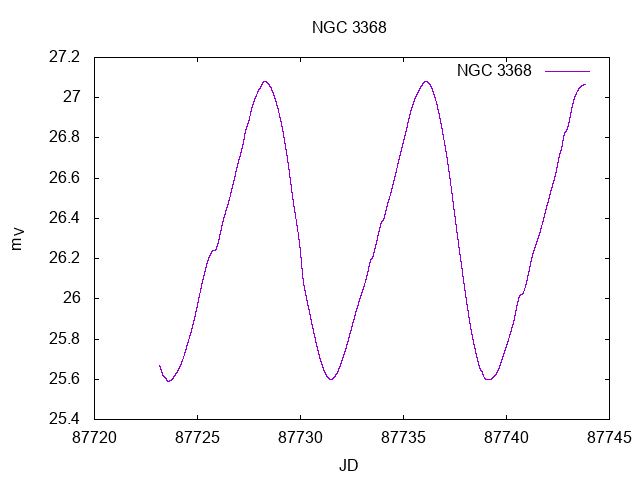
\includegraphics[width=.7\textwidth]{Codice/data/10_NGC3368.png}
  \caption{Curva di Luce della Cefeide in NGC3368.}
\end{figure}

\paragraph{NGC 3621}
\begin{center}
  \begin{tabular}{cccc}
  \toprule
  Periodo Medio ($JD$) & Errore Periodo ($JD$) & M. Apparente Media &
                                                                  Errore
                                                                      su
                                                                      M.A. \\
  \midrule
  $20.12$ & $6.41\e{-2}$ & $24.12$ & $3.47\e{-1}$ \\
  \bottomrule
 \end{tabular}
\end{center}

\begin{figure}[H]
  \centering
  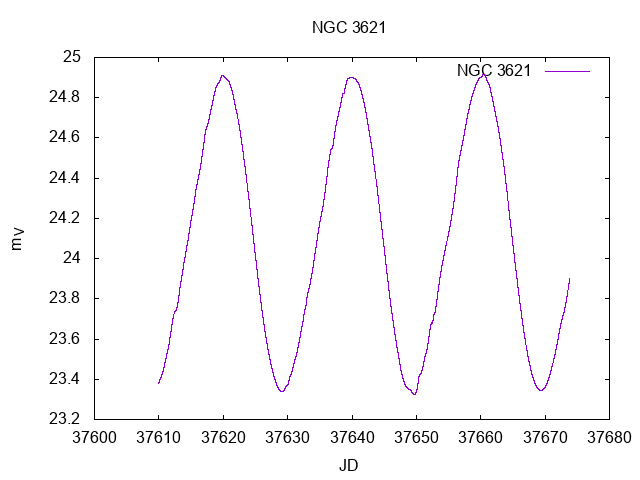
\includegraphics[width=.7\textwidth]{Codice/data/11_NGC3621.png}
  \caption{Curva di Luce della Cefeide in NGC3621.}
\end{figure}

\paragraph{NGC 4321}
\begin{center}
  \begin{tabular}{cccc}
  \toprule
  Periodo Medio ($JD$) & Errore Periodo ($JD$) & M. Apparente Media &
                                                                  Errore
                                                                      su
                                                                      M.A. \\
  \midrule
  $28.18$ & $9.61\e{-2}$ & $25.50$ & $2.36\e{-1}$ \\
  \bottomrule
 \end{tabular}
\end{center}

\begin{figure}[H]
  \centering
  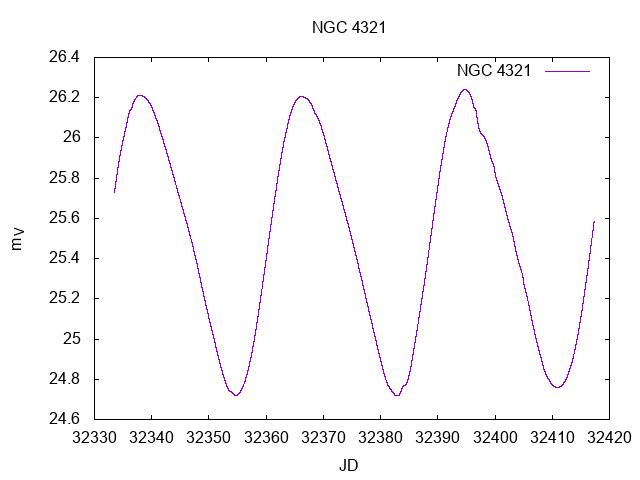
\includegraphics[width=.7\textwidth]{Codice/data/12_NGC4321.png}
  \caption{Curva di Luce della Cefeide in NGC4321.}
\end{figure}

\paragraph{NGC 4496}
\begin{center}
  \begin{tabular}{cccc}
  \toprule
  Periodo Medio ($JD$) & Errore Periodo ($JD$) & M. Apparente Media &
                                                                  Errore
                                                                      su
                                                                      M.A. \\
  \midrule
  $22.15$ & $4.57\e{-2}$ & $26.75$ & $1.74\e{-1}$ \\
  \bottomrule
 \end{tabular}
\end{center}

\begin{figure}[H]
  \centering
  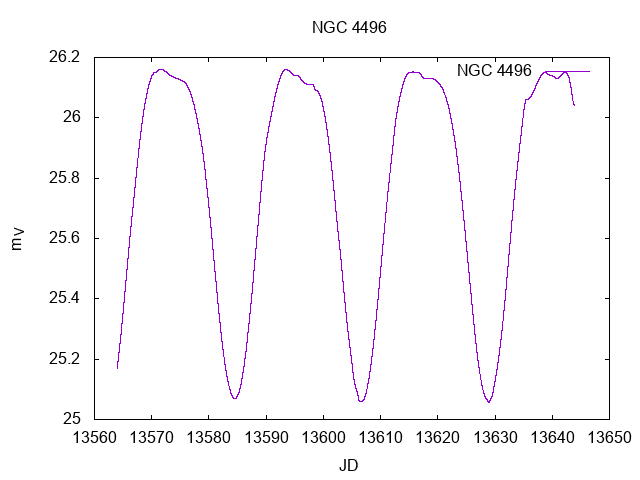
\includegraphics[width=.7\textwidth]{Codice/data/13_NGC4496.png}
  \caption{Curva di Luce della Cefeide in NGC4496.}
\end{figure}

\paragraph{NGC 4548}
\begin{center}
  \begin{tabular}{cccc}
  \toprule
  Periodo Medio ($JD$) & Errore Periodo ($JD$) & M. Apparente Media &
                                                                  Errore
                                                                      su
                                                                      M.A. \\
  \midrule
  $6.98$ & $2.19\e{-1}$ & $27.40$ & $2.29\e{-1}$ \\
  \bottomrule
 \end{tabular}
\end{center}

\begin{figure}[H]
  \centering
  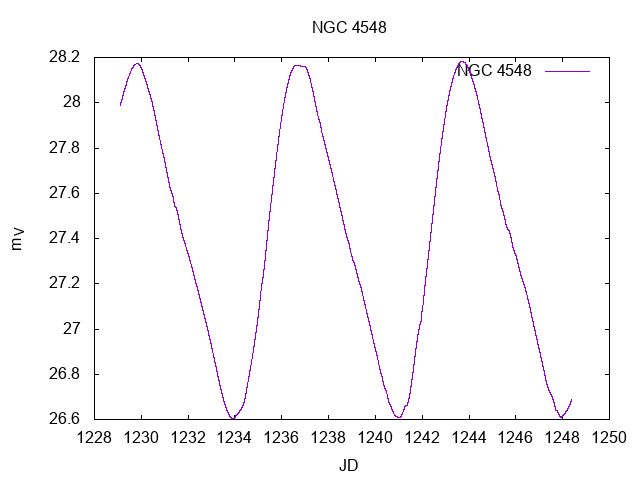
\includegraphics[width=.7\textwidth]{Codice/data/14_NGC4548.png}
  \caption{Curva di Luce della Cefeide in NGC4548.}
\end{figure}

\paragraph{NGC 4535}
\begin{center}
  \begin{tabular}{cccc}
  \toprule
  Periodo Medio ($JD$) & Errore Periodo ($JD$) & M. Apparente Media &
                                                                  Errore
                                                                      su
                                                                      M.A. \\
  \midrule
  $8.42$ & $5.31\e{-3}$ & $27.10$ & $3.75\e{-1}$ \\
  \bottomrule
 \end{tabular}
\end{center}

\begin{figure}[H]
  \centering
  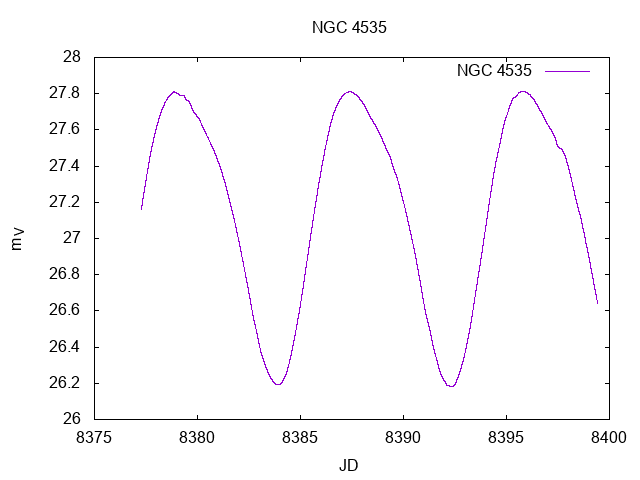
\includegraphics[width=.7\textwidth]{Codice/data/15_NGC4535.png}
  \caption{Curva di Luce della Cefeide in NGC4535.}
\end{figure}

\paragraph{NGC 4536}
\begin{center}
  \begin{tabular}{cccc}
  \toprule
  Periodo Medio ($JD$) & Errore Periodo ($JD$) & M. Apparente Media &
                                                                  Errore
                                                                      su
                                                                      M.A. \\
  \midrule
  $16.15$ & $7.50\e{-2}$ & $26.16$ & $3.40\e{-1}$ \\
  \bottomrule
 \end{tabular}
\end{center}

\begin{figure}[H]
  \centering
  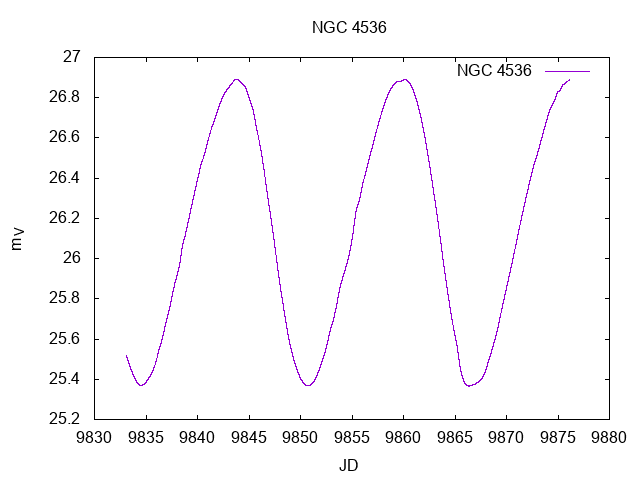
\includegraphics[width=.7\textwidth]{Codice/data/16_NGC4536.png}
  \caption{Curva di Luce della Cefeide in NGC4536.}
\end{figure}

\paragraph{NGC 4639}
\begin{center}
  \begin{tabular}{cccc}
  \toprule
  Periodo Medio ($JD$) & Errore Periodo ($JD$) & M. Apparente Media &
                                                                  Errore
                                                                      su
                                                                      M.A. \\
  \midrule
  $32.44$ & $1.31\e{-1}$ & $26.12$ & $7.72\e{-2}$ \\
  \bottomrule
 \end{tabular}
\end{center}

\begin{figure}[H]
  \centering
  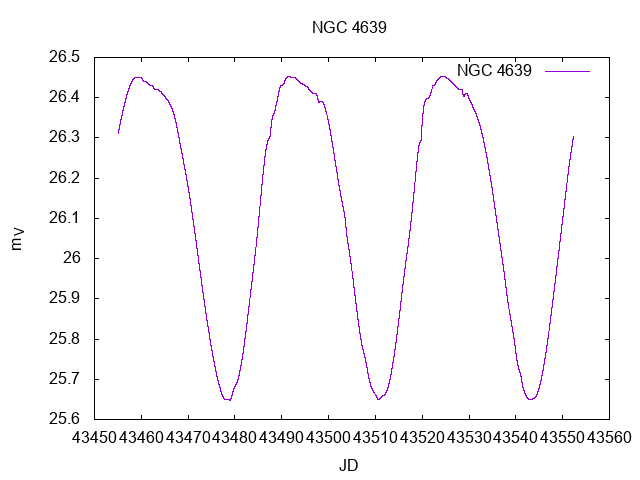
\includegraphics[width=.7\textwidth]{Codice/data/17_NGC4639.png}
  \caption{Curva di Luce della Cefeide in NGC4639.}
\end{figure}

\paragraph{NGC 4725}
\begin{center}
  \begin{tabular}{cccc}
  \toprule
  Periodo Medio ($JD$) & Errore Periodo ($JD$) & M. Apparente Media &
                                                                  Errore
                                                                      su
                                                                      M.A. \\
  \midrule
  $16.66$ & $3.44\e{-2}$ & $25.71$ & $3.21\e{-1}$ \\
  \bottomrule
 \end{tabular}
\end{center}

\begin{figure}[H]
  \centering
  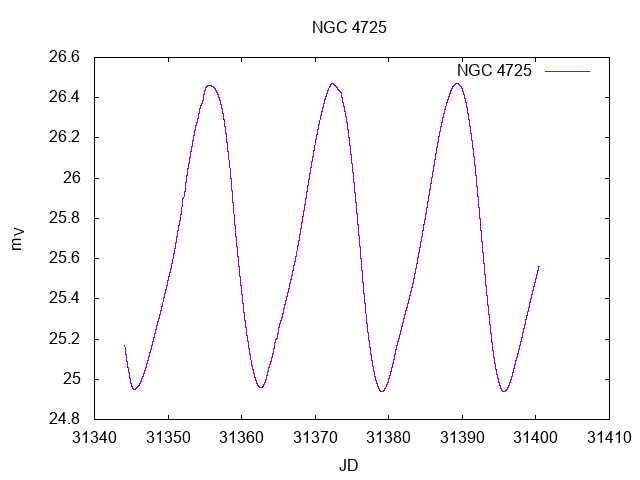
\includegraphics[width=.7\textwidth]{Codice/data/18_NGC4725.png}
  \caption{Curva di Luce della Cefeide in NGC4725.}
\end{figure}

\paragraph{NGC 7331}
\begin{center}
  \begin{tabular}{cccc}
  \toprule
  Periodo Medio ($JD$) & Errore Periodo ($JD$) & M. Apparente Media &
                                                                  Errore
                                                                      su
                                                                      M.A. \\
  \midrule
  $13.83$ & $2.16\e{-1}$ & $26.33$ & $4.63\e{-2}$ \\
  \bottomrule
 \end{tabular}
\end{center}

\begin{figure}[H]
  \centering
  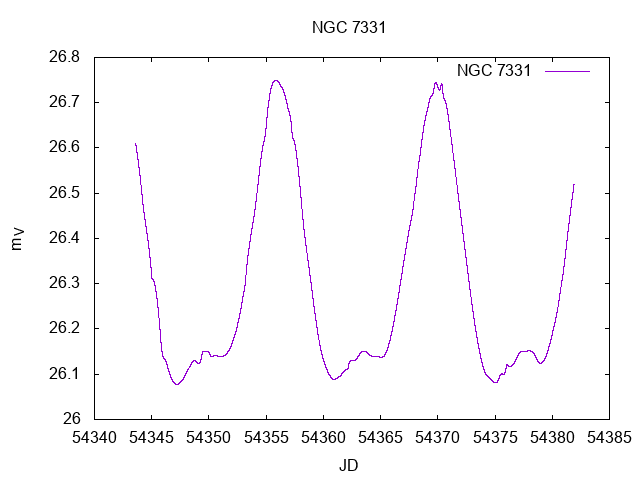
\includegraphics[width=.7\textwidth]{Codice/data/19_NGC7331.png}
  \caption{Curva di Luce della Cefeide in NGC7331.}
\end{figure}

\subsection{Magnitudine Assoluta}

Sfruttando la relazione Periodo-Luminosità, con i valori per i
coefficienti trovati a inizio codice, posso ottenere una stima della
magnitudine assoluta della stella e del suo errore.

\begin{equation}
  M_V = -2.90 \log (P) -1.21
\end{equation}

Ne calcolo l'errore inserendo:
\begin{equation}
  dM_V = \frac{-2.90}{P} \log{dP}
 \end{equation}

\begin{center}
  \begin{tabular}{ccc}
  \toprule
  Cefeide (nome Galassia) & Magnitudine Assoluta & Errore Magnitudine\\
  \midrule
    NGC0925 & $-4.27$ & $4.07\e{-1}$ \\
    NGC1326 & $-3.93$ & $4.40\e{-1}$ \\
    NGC1365 & $-5.06$ & $1.05\e{-1}$ \\
    NGC1425 & $-4.20$ & $4.62\e{-1}$ \\
    NGC2403 & $-2.89$ & $1.56$ \\
    NGC2541 & $-4.94$ & $7.73\e{-2}$ \\
    NGC2090 & $-5.12$ & $1.94\e{-1}$ \\
    NGC3198 & $-4.63$ & $2.21\e{-1}$ \\
    NGC3351 & $-3.86$ & $6.36\e{-1}$ \\
    NGC3368 & $-3.78$ & $4.76\e{-1}$ \\
    NGC3521 & $-4.99$ & $1.72\e{-1}$ \\
    NGC4321 & $-5.41$ & $1.05\e{-1}$ \\
    NGC4496 & $-5.11$ & $1.75\e{-1}$ \\
    NGC4548 & $-3.65$ & $2.74\e{-1}$ \\
    NGC4535 & $-3.89$ & $7.84\e{-1}$ \\
    NGC4536 & $-4.71$ & $2.02\e{-1}$ \\
    NGC4639 & $-5.59$ & $7.91\e{-2}$ \\
    NGC4725 & $-4.75$ & $2.55\e{-1}$ \\
    NGC7331 & $-4.51$ & $1.40\e{-1}$ \\
  \bottomrule
 \end{tabular}
\end{center}

\subsection{Distanza della Galassia}

Utilizzando il valore trovato della magnitudine assoluta, posso
trovare dapprima il modulo di distanza:

\begin{equation}
  \begin{cases}
    \mu = m_V - M_v \\
    d\mu = \sqrt{dm_V^2, dM_V^2}
  \end{cases}
\end{equation}

per poi ottenere la distanza (della galassia ospitante). Divido per
$10^6$ per ottenere la distanza in $Mpc$.

\begin{equation}
  \begin{cases}
    D = \frac{10*{0.2\mu +1}}{10^6} \\
    dD = \frac{4.61\; e^{0.461\cdot \mu} d\mu}{10^6}
  \end{cases}
\end{equation}

    

Riporto direttamente le distanze delle galassie 

\begin{center}
  \begin{tabular}{ccc}
  \toprule
  Cefeide (nome Galassia) & Distanza ($Mpc$) & Errore Distanza ($Mpc$)
    \\
  \midrule
    NGC0925 & $9.14$ & $1.93$ \\
    NGC1326 & $16.14$ & $3.35$ \\
    NGC1365 & $17.89$ & $1.03$ \\
    NGC1425 & $21.83$ & $4.98$ \\
    NGC2403 & $3.23$ & $2.41$ \\
    NGC2541 & $11.15$ & $0.41$ \\
    NGC2090 & $11.73$ & $1.41$ \\
    NGC3198 & $13.76$ & $2.06$ \\
    NGC3351 & $9.99$ & $3.75$ \\
    NGC3368 & $10.51$ & $2.74$ \\
    NGC3521 & $6.63$ & $1.20$ \\
    NGC4321 & $15.18$ & $1.84$ \\
    NGC4496 & $14.83$ & $1.71$ \\
    NGC4548 & $16.22$ & $2.71$ \\
    NGC4535 & $15.77$ & $6.41$ \\
    NGC4536 & $14.91$ & $2.76$ \\
    NGC4639 & $21.95$ & $1.14$ \\
    NGC4725 & $12.34$ & $2.37$ \\
    NGC7331 & $14.74$ & $1.01$ \\
  \bottomrule
 \end{tabular}
\end{center}

\subsection{Costante di Hubble}

Calcolando la costante di Hubble utilizzando la distanza in $Mpc$
appena trovata e usando la velocità di recessione del file fornito con
l'esercizio:

\begin{equation}
  \begin{cases}
    H_0 = \frac{v_{rec}}{D} \\
    dH_0 = \sqrt{ \left ( \frac{dv}{D} \right )^2 + \left (
        \frac{v}{D^2} dD \right ) ^2}
    \end{cases}
  \end{equation}

  Ottengo i seguenti valori:

  \begin{center}
  \begin{tabular}{ccc}
  \toprule
  Cefeide (nome Galassia) & $H_0$ ($\frac{km}{s\cdot Mpc}$) & $dH_0$
                                                             ($\frac{km}{s
                                                             \cdot Mpc}$)
    \\
  \midrule
    NGC0925 & $72.68$ & $35.26$ \\
    NGC1326 & $111.1$ & $45.30$ \\
    NGC1365 & $89.10$ & $24.96$ \\
    NGC1425 & $67.48$ & $15.42$ \\
    NGC2403 & $86.16$ & $69.58$ \\
    NGC2541 & $64.06$ & $20.06$ \\
    NGC2090 & $75.19$ & $9.80$ \\
    NGC3198 & $56.11$ & $10.07$ \\
    NGC3351 & $64.24$ & $58.52$ \\
    NGC3368 & $73.07$ & $48.60$ \\
    NGC3521 & $91.91$ & $64.22$ \\
    NGC4321 & $94.39$ & $11.42$ \\
    NGC4496 & $95.99$ & $11.45$ \\
    NGC4548 & $85.31$ & $14.44$ \\
    NGC4535 & $91.58$ & $37.29$ \\
    NGC4536 & $95.46$ & $17.85$ \\
    NGC4639 & $63.92$ & $3.89$ \\
    NGC4725 & $89.37$ & $19.78$ \\
    NGC7331 & $67.78$ & $13.01$ \\
  \bottomrule
 \end{tabular}
\end{center}

Con tutti questi valori procedo con il determinare una media pesata
usando come pesi:

\begin{equation*}
  p_i = \frac{1}{dH_{0,i}^2}
\end{equation*}

Ottengo così una costante di Hubble:

\begin{equation}
  \begin{cases}
    H_0 = 71.09 \, \frac{km}{s\cdot Mpc} \\
    dH_0 = 2.78 \, \frac{km}{s \cdot Mpc}
  \end{cases}
\end{equation}

\subsection{Modelli Cosmologici}

Utilizzando il valore della costante di Hubble così ottenuta, posso
calcolare le coppie di parametri cosmologici $\Omega_M$ e
$\Omega_\Lambda$ che rendono l'età dell'universo pari a $t_0 = 13.82
\pm 0.1382$.

\paragraph{Universo Piatto}

Dapprima scelgo di analizzare un universo con geometria Piatta, in cui
\begin{equation*}
  \Omega = \Omega_M + \Omega_\Lambda = 1
\end{equation*}

Tramite il codice ottengo tre coppie di parametri rispettivamente per
il valore medio di $H_0$, il suo valore massimo e il suo valore
minimo.

\begin{equation}
  \begin{cases}
    H_{0,mean} : \qquad \Omega_M = 0.254 \qquad \Omega_L = 0.746 \\
    H_{0,max} : \qquad \Omega_M = 0.220 \qquad \Omega_L = 0.780 \\
    H_{0,min} : \qquad \Omega_M = 0.293 \qquad \Omega_L = 0.707
  \end{cases}
\end{equation}

  A questo va confrontato un valore utilizzando i dati di
  \emph{Planck}, usando la \textbf{CMB}:
  $$ H_0 = 67.4 $$
  $$ dH_0 = 0.5 $$

  \begin{equation}
  \begin{cases}
    H_{0,mean} : \qquad \Omega_M = 0.308 \qquad \Omega_L = 0.692 \\
    H_{0,max} : \qquad \Omega_M = 0.300 \qquad \Omega_L = 0.700 \\
    H_{0,min} : \qquad \Omega_M = 0.316 \qquad \Omega_L = 0.684
  \end{cases}
\end{equation}

Con i dati del team \emph{SH0ES} usando le Supernovae:

\begin{equation}
  \begin{cases}
    H_{0,mean} : \qquad \Omega_M = 0.224 \qquad \Omega_L = 0.776\\
    H_{0,max} : \qquad \Omega_M = 0.209 \qquad \Omega_L = 0.791 \\
    H_{0,min} : \qquad \Omega_M = 0.241 \qquad \Omega_L = 0.759
  \end{cases}
\end{equation}

\paragraph{Universo Aperto}

Proseguo con il calcolo per un universo aperto, dove cioè $\Omega <
1$. Utilizzando la costante di Hubble derivata dal mio codice ottengo:

\begin{equation}
  \begin{cases}
    H_{0,mean} : \qquad \Omega_M = 0.119 \qquad \Omega_L = 0.445 \\
    H_{0,max} : \qquad \Omega_M = 0.198 \qquad \Omega_L = 0.733 \\
    H_{0,min} : \qquad \Omega_M = 0.052 \qquad \Omega_L = 0.132
  \end{cases}
\end{equation}

Usando i dati della missione Planck (CMB):

\begin{equation}
  \begin{cases}
    H_{0,mean} : \qquad \Omega_M = 0.109 \qquad \Omega_L = 0.254 \\
    H_{0,max} : \qquad \Omega_M = 0.163 \qquad \Omega_L = 0.411 \\
    H_{0,min} : \qquad \Omega_M = 0.223 \qquad \Omega_L = 0.497
  \end{cases}
\end{equation}

Usando i dati del team SH0ES (SN):

\begin{equation}
  \begin{cases}
    H_{0,mean} : \qquad \Omega_M = 0.046 \qquad \Omega_L = 0.328 \\
    H_{0,max} : \qquad \Omega_M = 0.083 \qquad \Omega_L = 0.490 \\
    H_{0,min} : \qquad \Omega_M = 0.104 \qquad \Omega_L = 0.446
  \end{cases}
\end{equation}

\paragraph{Universo Chiuso}

Infine, calcolo le coppie di parametri cosmologici che calcolino
un'età dell'universo pari a $13.82\pm0.1382$ per un universo che abbia
geometria chiusa. Cioè, tali per cui $\Omega > 1$.

Usando i miei valori:
\begin{equation}
  \begin{cases}
    H_{0,mean} : \qquad \Omega_M = 0.276 \qquad \Omega_L = 0.790 \\
    H_{0,max} : \qquad \Omega_M = 0.294 \qquad \Omega_L = 0.926 \\
    H_{0,min} : \qquad \Omega_M = 0.332 \qquad \Omega_L = 0.780
  \end{cases}
\end{equation}

Usando i dati di Planck:

\begin{equation}
  \begin{cases}
    H_{0,mean} : \qquad \Omega_M = 0.446 \qquad \Omega_L = 0.941 \\
    H_{0,max} : \qquad \Omega_M = 0.393 \qquad \Omega_L = 0.872 \\
    H_{0,min} : \qquad \Omega_M = 0.407 \qquad \Omega_L = 0.850
  \end{cases}
\end{equation}

Infine, usando i dati di SH0ES:

\begin{equation}
  \begin{cases}
    H_{0,mean} : \qquad \Omega_M = 0.287 \qquad \Omega_L = 0.900 \\
    H_{0,max} : \qquad \Omega_M = 0.294 \qquad \Omega_L = 0.960 \\
    H_{0,min} : \qquad \Omega_M = 0.242 \qquad \Omega_L = 0.761
  \end{cases}
\end{equation}

\section{Discussione e Problemi}

I calcoli effettuati dal mio codice generano un risultato coerente con
le derivazioni fatte dalle missioni Planck e dal team SH0ES.

La precisione nel calcolo dei periodi e delle luminosità è buona, ma
non superba. Questo però non pregiudica un buon risultato.

La maggior parte dell'errore accumulato (errore che appare visibile nella tabella
relativa alle costanti di Hubble derivate con le singole Cefeidi)
proviene sicuramente dal calcolo delle distanze.

Essendo prodotto da una legge esponenziale del modulo di distanza, la
distanza vede un aumento importante (ma verosimilmente intrinseco)
dell'errore. Mediando tante misure, come ho fatto qui, si riesce a
ottenere un valore per la costante di Hubble che comunque presenta una
incertezza decente, ma da questo si può facilmente capire perchè gli
Astrofisici spingono continuamente per la costruzione e la messa in
orbita di satelliti con precisione crescente.

Il secondo termine che aumenta l'errore, probabilmente, è la
precisione della velocità di recessione. Per alcuni valori, infatti,
l'incertezza è addirittura dell'ordine dell'$70-80\%$.

\subsection{Difetto del Codice}

Il grosso difetto del codice che ho scritto è l'efficienza. Per
svolgere l'intero codice su macOS 10.14.6 con una CPU $i7 - 4578U$ e
RAM $16GB$ impiega $24m41.700$!

Sicuramente si potrebbe migliorare l'efficienza del codice
architettando il calcolo non su array come ho fatto io, ma usando
scalari o qualche vettore meno dimensionale rispetto a quelli che ho
usato io.

L'operazione più intensiva per la CPU sono, però, sicuramente le due condizioni per l'Universo Aperto o Universo
Chiuso. Il programma si trova davanti un pool di un milione di
possibili valori da controllare. Non sono riuscito a trovare nessuna
via analitica per semplificare il lavoro al codice. Le alternative che
avevo scritto, impiegavano anche più tempo.

\end{document}
